% !TEX TS-program = lualatex
%\documentclass[handout]{beamer}
\documentclass{beamer}
\input{../common/misomva}
\usepackage{fontawesome5}
\usetikzlibrary{positioning, shapes.geometric, shapes.symbols, shadows}
\begin{document}
% Topic-specific title slide
\newcommand{\topictitle}{Natural Graphs}
\newcommand{\topicsubtitle}{Social, Information, and Biological Networks}
\newcommand{\misoclasstinytitleslide}{Partially based on material by:  Andreas Krause, \\[-1em] Branislav Kveton, Michael Kearns}

\MakeTopicSlide

\begin{frame}
\frametitle{Natural graphs from \emphcol{social networks}}
\begin{columns}
\begin{column}{.5\textwidth}
\begin{itemize}[<+-| alert@+>]\addtolength{\itemsep}{1\baselineskip}
\item people and their interactions
\item structure is rather a \textit{phenomena}
\item typical ML tasks 
\begin{itemize}\addtolength{\itemsep}{0.5\baselineskip}
\item advertising 
%\item product placement 
\item link prediction (PYMK)
\item find influential sources 
\end{itemize}
\end{itemize}
\end{column}
\begin{column}{.5\textwidth}
\begin{center}
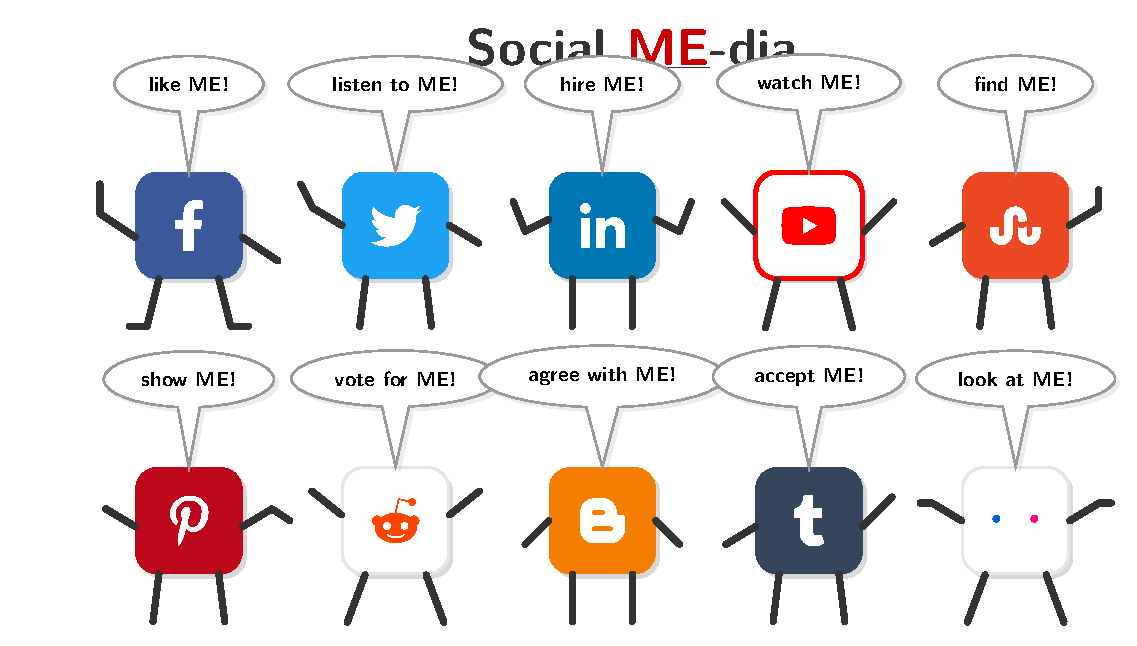
\includegraphics[width=\textwidth]{../img/mlapa-tikz-preview}
\end{center}
\end{column}
\end{columns}
\end{frame}

\begin{frame}
\frametitle{Success story \#1 \emphcol{Product placement} - problem}
\begin{center}
% Manual layout to avoid spring layout overlap (requires lualatex)
\begin{tikzpicture}[
  marked/.style={fill=black!50},
  nd/.style={circle, draw, minimum size=8mm, inner sep=0pt},
  lbl/.style={font=\small, fill=white, inner sep=1pt}
]
% Nodes
\node[nd, onslide=<3-| handout:3->{marked}] (A) at (0,2) {A};
\node[nd] (B) at (3,2) {B};
\node[nd, onslide=<6-| handout:6->{marked}] (C) at (1.5,0) {C};
\node[nd, onslide=<8-| handout:8->{marked}] (D) at (0,-2) {D};
\node[nd] (E) at (3,-2) {E};
\node[nd] (F) at (1.5,-4) {F};
% Edges with overlay colors
\only<1| handout:1>{\draw (A)--(B); \draw (A)--(C); \draw (B)--(C); \draw (C)--(D); \draw (D)--(E); \draw (D)--(F); \draw (F)--(E);}
\only<2-3| handout:2>{\draw (A)--node[lbl,above]{0.3}(B); \draw (A)--node[lbl,left]{0.5}(C); \draw (B)--node[lbl,right]{0.5}(C); \draw (C)--node[lbl,left]{0.5}(D); \draw (D)--node[lbl,above]{0.2}(E); \draw (D)--node[lbl,left]{0.2}(F); \draw (F)--node[lbl,right]{0.5}(E);}
\only<4| handout:3>{\draw[red] (A)--node[lbl,above]{0.3}(B); \draw (A)--node[lbl,left]{0.5}(C); \draw (B)--node[lbl,right]{0.5}(C); \draw (C)--node[lbl,left]{0.5}(D); \draw (D)--node[lbl,above]{0.2}(E); \draw (D)--node[lbl,left]{0.2}(F); \draw (F)--node[lbl,right]{0.5}(E);}
\only<5| handout:4>{\draw[red] (A)--node[lbl,above]{0.3}(B); \draw[green] (A)--node[lbl,left]{0.5}(C); \draw (B)--node[lbl,right]{0.5}(C); \draw (C)--node[lbl,left]{0.5}(D); \draw (D)--node[lbl,above]{0.2}(E); \draw (D)--node[lbl,left]{0.2}(F); \draw (F)--node[lbl,right]{0.5}(E);}
\only<6| handout:5>{\draw[red] (A)--node[lbl,above]{0.3}(B); \draw[green] (A)--node[lbl,left]{0.5}(C); \draw (B)--node[lbl,right]{0.5}(C); \draw (C)--node[lbl,left]{0.5}(D); \draw (D)--node[lbl,above]{0.2}(E); \draw (D)--node[lbl,left]{0.2}(F); \draw (F)--node[lbl,right]{0.5}(E);}
\only<7| handout:6>{\draw[red] (A)--node[lbl,above]{0.3}(B); \draw[green] (A)--node[lbl,left]{0.5}(C); \draw[red] (B)--node[lbl,right]{0.5}(C); \draw[green] (C)--node[lbl,left]{0.5}(D); \draw (D)--node[lbl,above]{0.2}(E); \draw (D)--node[lbl,left]{0.2}(F); \draw (F)--node[lbl,right]{0.5}(E);}
\only<8-9| handout:7-8>{\draw[red] (A)--node[lbl,above]{0.3}(B); \draw[green] (A)--node[lbl,left]{0.5}(C); \draw[red] (B)--node[lbl,right]{0.5}(C); \draw[green] (C)--node[lbl,left]{0.5}(D); \draw (D)--node[lbl,above]{0.2}(E); \draw (D)--node[lbl,left]{0.2}(F); \draw (F)--node[lbl,right]{0.5}(E);}
\only<9| handout:8>{\draw[red] (D)--node[lbl,above]{0.2}(E);}
\only<10-| handout:9->{\draw[red] (A)--node[lbl,above]{0.3}(B); \draw[green] (A)--node[lbl,left]{0.5}(C); \draw[red] (B)--node[lbl,right]{0.5}(C); \draw[green] (C)--node[lbl,left]{0.5}(D); \draw[red] (D)--node[lbl,above]{0.2}(E); \draw[red] (D)--node[lbl,left]{0.2}(F); \draw[red] (F)--node[lbl,right]{0.5}(E);}
\end{tikzpicture}
\end{center}
\onslide<2-| handout:2->{
\textbf{Who should get free cell phones?} \moves
$V$ = \{\textbf{A}lice,\textbf{B}ob,\textbf{C}harlie,\textbf{D}orothy,\textbf{E}ric,\textbf{F}iona\}
\moves}

\onslide<10-| handout:10->{
$F(S)$ = Expected number of people influenced when targeting $S\subseteq V$
under some propagation model - e.g., cascades
}

\onslide<11-| handout:10->{
\bigskip
\questionbox{How would you choose the target customers?}\\
}
\onslide<12-| handout:10->{
\notecol{\tiny \qquad highest degree, close to the center, $\dots$}
}
\onslide<1-| handout:1->
{\tiny \flushright
Maximizing the Spread of Influence through a Social Network
\url{http://www.cs.cornell.edu/home/kleinber/kdd03-inf.pdf}
}

\end{frame}


\MakeLastSlide
\end{document}
